\chapter{Application Architecture}
\section{Overview}
This chapter describes application architecture which was purpose of this thesis. Application is organized into \textbf{four} essential parts:
\begin{itemize}
	\item Data source: loadstone DBMS
	\item Module 1: loadstone-model
	\item Module 2: loadstone-api
	\item Module 3: loadstone-package
\end{itemize}

\textit{Note: naming convention can differ from standard UML definitions. Module can be considered as component - represents a modular part of a system, that encapsulates its content and whose manifestation is replaceable within its environment. A component defines its behaviour in terms of provided and required interfaces \cite{22}. Module convention comes from the fact that application life-cycle and dependency management is marshalled by tool \textbf{Maven}. Maven uses naming convention of modules and helps developer to avoid introducing circular dependencies so application is easier to maintain in future} \cite{23}.

\section{Architecture scheme}
In the figure \ref{fig:@=architecture} is depicted overall architecture of Loadstone application.
\begin{figure}
	\centering
	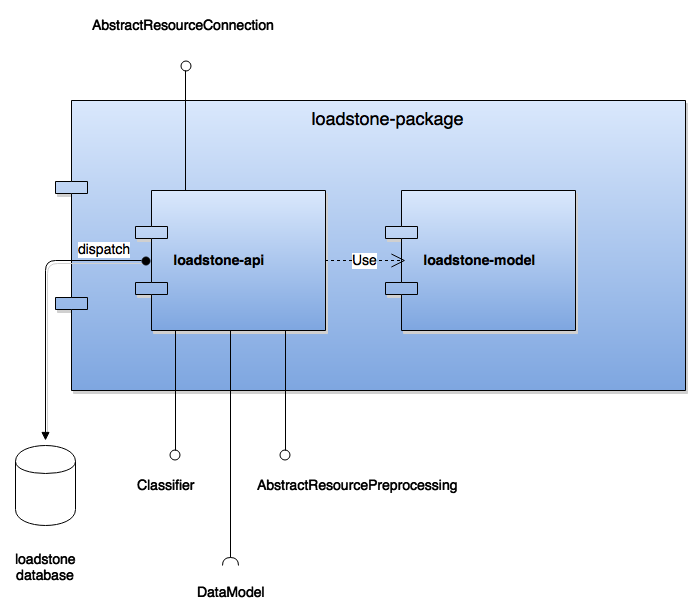
\includegraphics[scale=0.6]{architecture.png}
	\caption{Loadstone application architecture}
	\label{fig:@=architecture}
\end{figure}

\section{Architecture UML Class diagram}
To explore more implementation of application figure \ref{fig:@=loadstone_uml} should be analysed. It clearly describes technical details of application.
\begin{figure}
	\centering
	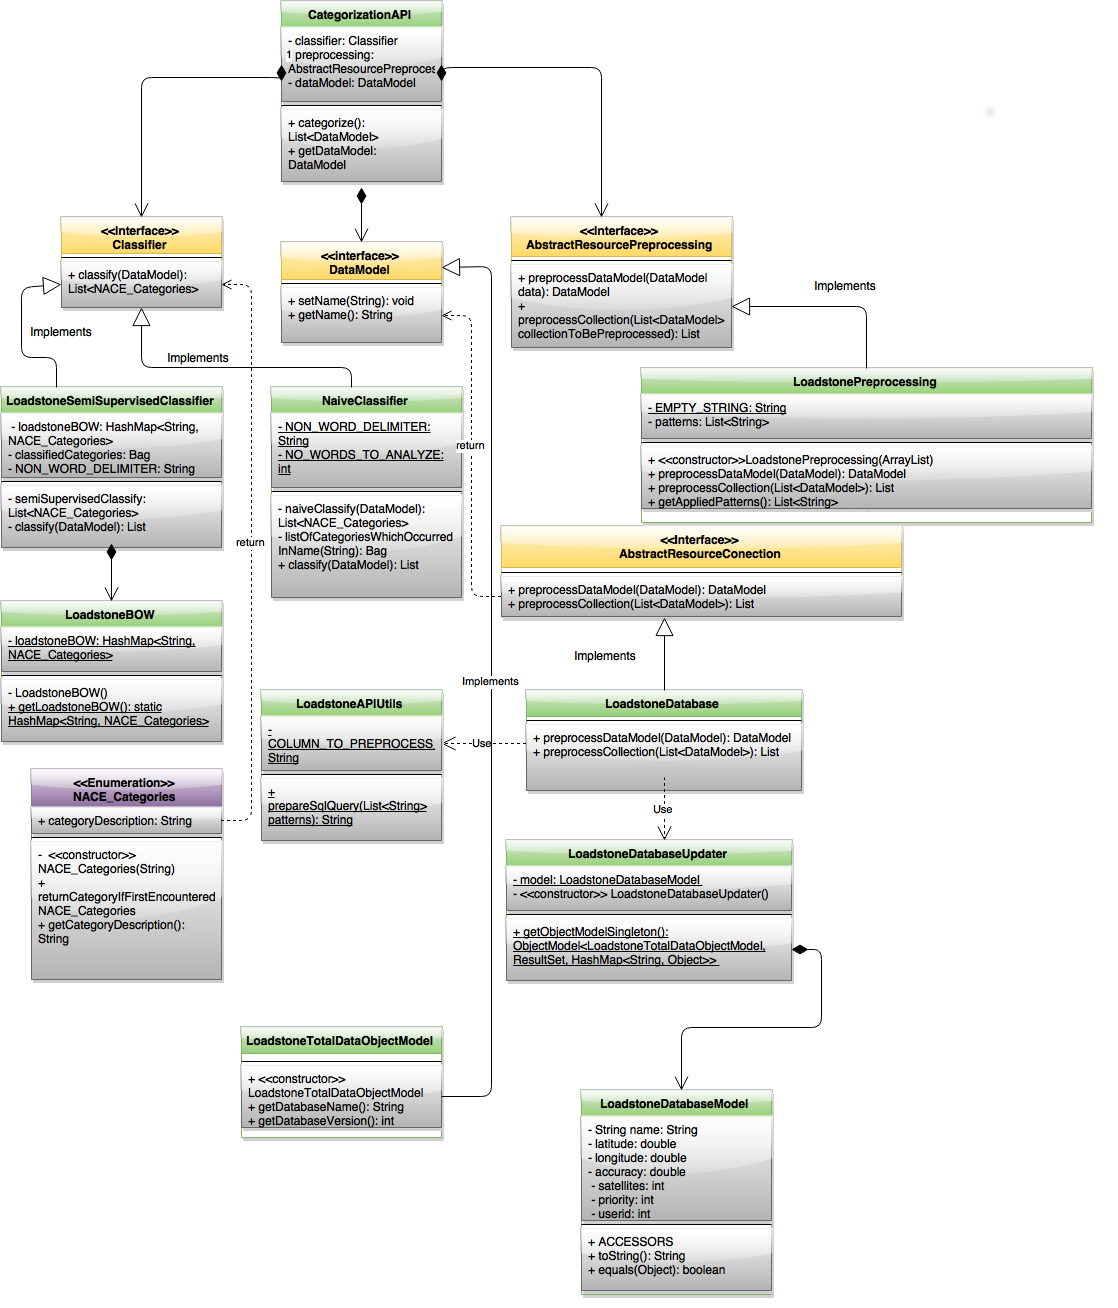
\includegraphics[scale=0.4]{UML.png}
	\caption{Loadstone application UML Class Diagram}
	\label{fig:@=loadstone_uml}
\end{figure}

\section{POI Categories}

\subsection{Tendency in POI categories}
To effectively categorize POI there has to be defined appropriate category hierarchy. There are a lot of multiple standards which are widely used in many different solutions and technologies. Unfortunately there is no world-wide standard defined for POI categories. More frequent observation can be done when looking at companies like: \textbf{Garmin, TomTom, Waze} that those entities try to introduce their own solutions. Garmin offers its own \textit{POILoader} which allows for own category definition \cite{9}. On the other hand TomTom offers 500 different POI categories by default but if user is eager to add custom POIs additional steps need to be done \cite{10}. User must prepare his own files with extension \textbf{\textit{.ov2}} and deploy it on GPS device. What is more deployment process depend on device model. Waze also defines it's own POI category standard \cite{14}. There is an endeavour done by \textbf{W3C} organization about POI Data Model standard (figure: \ref{fig:@=w3cDataModel}). Unfortunately according do W3C wiki it is still in beta version and categories are supposed to be defined in future \cite{12}. Only XML standard was developed (which supposed to be used as world-wide standard for POI data transfer) \cite{13}.
\begin{figure}[h]
	\centering
	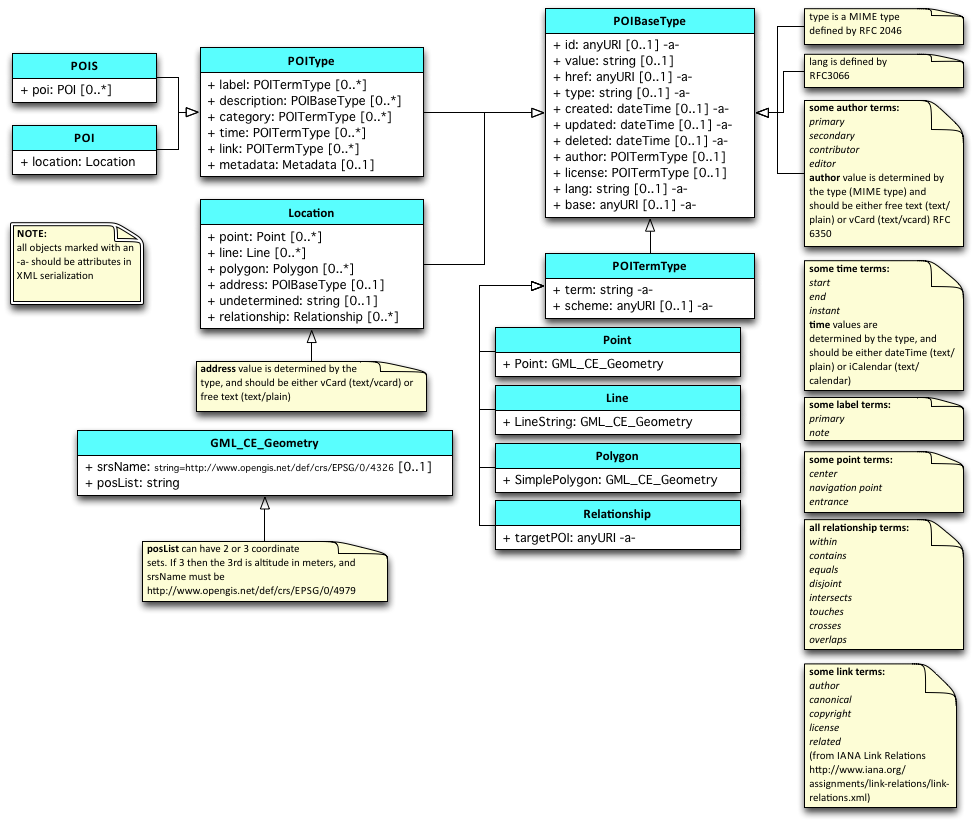
\includegraphics[scale=0.5]{W3c_poi_model.png}
	\caption{W3C UML Diagram POI Data Model}
	\label{fig:@=w3cDataModel}
\end{figure}
There is an apprehensible delamination in field of POI categories. It is difficult to find a standard which could be useful and well known for every data source. Fortunately there are standards defined by governments which describe categories in very detailed way and have endorsement by substantive position as countries governments possess. 
\subsection{NAICS}
\textit{\textbf{The North American Industry Classification System (NAICS)}} widely used in countries of North America. Developed by three organizations:  U.S. Economic Classification Policy Committee (ECPC), Statistics Canada, Mexico's Instituto Nacional de Estadistica y Geografia. It is mainly used by Federal agencies to collect data about business entities for statistic purposes. It is successor of \textit{\textbf{Standard Industrial Classification (SIC)}}. NAICS classification is basing on codes which correspond to category description. Code can at most consist of six digits (the more digits included in code the more detailed category description is). Latest NAICS revision was issued in 2012 \cite{15} \cite{16}.
\subsection{NACE}
\label{NACE}
\textit{\textbf{Statistical Classification of Economic Activities in the European Community (in French: Nomenclature statistique des activités économiques dans la Communauté européenne) - NACE}} system widely used in European Union. Similarly to NACE it is using combination of codes and category description. Code consists of letter and digits and creates special hierarchy of: sections, divisions, groups and classes. Section is marked by letter, division by two digits, groups and classes by one digit consecutively. Latest NACE revision (Rev.2) was issued in 2008 as a result of constantly developing and  newly appearing organizations especially in telecommunication business \cite{17} \cite{18}. Because Java application which is purpose of this thesis was developed in Poland NACE categorization standard was chosen to apply in it. Obviously information included in NACE are definitely too much detailed to be applied for POI categorization system so only main sections were taken into consideration \cite{31}. Assignment of category and description is presented in table \ref{tab:NaceMatching}.
\begin{table}[H] 
	\begin{tabular}{ | c | c |}
		\hline
		Category & Description\tabularnewline \hline
		A & Agriculture, forestry and fishing\\\hline
		B & Mining and quarrying\\\hline
		C & Manufacturing\\\hline
		D & Electricity, gas, steam and air conditioning supply\\\hline
		E & Water supply, sewerage, waste management and remediation activities\\\hline
		F & Construction\\\hline
		G & Wholesale and retail trade, repair of motor vehicles and motorcycles\\\hline
		H & Transporting and storage\\\hline
		I & Accommodation and food service activities\\\hline
		J & Information and communication\\\hline
		K & Financial and insurance activities\\\hline
		L & Real estate activities\\\hline
		M & Professional, scientific and technical activities\\\hline
		N & Administrative and support service activities\\\hline
		O & Public administration and defence, compulsory social security\\\hline
		P & Education\\\hline
		Q & Human health and social work activities\\\hline
		R & Arts, entertainment and recreation\\\hline
		S & Other services activities\\\hline
		T & \begin{tabular}{@{}c@{}}Activities of households as employers undifferentiated goods and services\\ - producing activities of households for own use\end{tabular}\\\hline
		U & Activities of extraterritorial organisations and bodies\\\hline
		NOT\_CLASSIFIED & Not classified\\ 		
		\hline
	\end{tabular}
	\caption{Implemented NACE categories with assigned human readable description}
	\label{tab:NaceMatching}
\end{table} 

\section{Java library as categorization API}
Main purpose of Java categorization API is to deliver an interface which would allow for convenient, correct and efficient results. API should be independent of data type which will be delivered. API responsibility is to enable functionalities (as this thesis states - categorization). To assure independence of data sources powerful mechanism of Java interfaces can be used - such approach introduce level of abstraction and allow Java library for easy communication with data sources. Java has very useful feature of importing and using libraries - when whole code is compiled to bytecode classes are bundled into resultant \textbf{\textit{.jar}} file - it can be immediately used in another Java project by another programmer. Moreover, resultant Java library project can be compiled with dependencies so programmer who will use library later will not have to bother about classes which were used during library development are were not part of Java API \cite{19}. This approach increases size of \textbf{\textit{.jar}} file but release user from inconvenient dependencies downloading and importing into project.    

\subsection{Packages organization}
API is divided into three packages: \textit{connection, classification} and \textit{utils}. Such packaging organization assures clear and concise representation of API functionalites and utilities. Functional packages are divided into similar hierarchy to interfaces and packages responsible for particular data source handling (figure \ref{fig:@=packages_oragnization}). For purpose of this thesis these packages were named \textit{Loadstone}. Obviously unit tests for corresponding executing classes are located into separate directory (according to maven directory structure) but are included in the same packages (for Java it is counterpart of namespace) \cite{20}.
\begin{figure}[h]
	\centering
	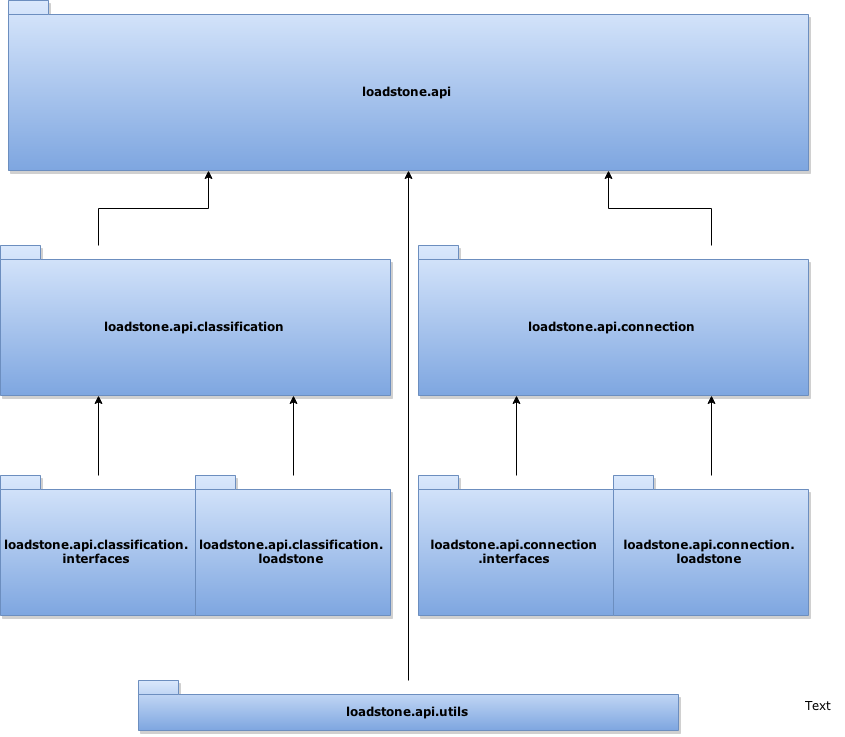
\includegraphics[scale=0.5]{loadstone_api_packages.png}
	\caption{Loadstone API packages organization}
	\label{fig:@=packages_oragnization}
\end{figure}
\subsection{Interface \newline loadstone.api.classification.interfaces.\newline AbstractResourcePreprocessing}
As mentioned before independence of input data is absolutely compulsory for API. To define preprocessing for each different kind of data source  AbstractResourcePreprocessing interface was defined. Classes which will be strictly delegated to pre-process particular source of data by implementation of this interface will be able to communicate with API and pass already preprocessed data for further classification methods.Interface also relies on model object data (DataModel) which is defined in another module of the project - \textbf{loadstone-model}. This assures for uniform and scalable solution for next data resources. AbstractResourcePreprocessing defines two methods which has to be implemented by data source dedicated classes to use categorization methods. Interface organization is depicted in the figure \ref{fig:@=AbstractResourcePreprocessing}:
\begin{figure}[h]
	\centering
	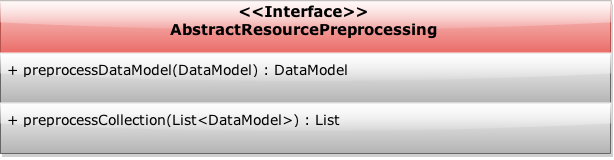
\includegraphics[scale=0.5]{AbstractResourcePreprocessing.png}
	\caption{AbstractResourcePreprocessing UML Diagram}
	\label{fig:@=AbstractResourcePreprocessing}
\end{figure}
\subsection{Interface \newline loadstone.api.classification.Classifier}
This interface is devoted for classes implementing classification functionalities. It imposes on classes to deliver data source in appropriate way and return List. Main idea of this interface is to inform user that every data model object can be assigned to one or more classes. UML diagram on figure \ref{fig:@=classifier}.
\begin{figure}[h]
	\centering
	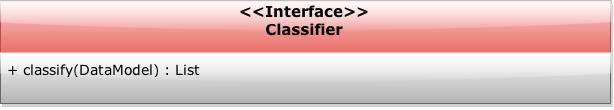
\includegraphics[scale=0.5]{classifier_interface.png}
	\caption{Interface Classifier UML Diagram}
	\label{fig:@=classifier}
\end{figure}
\subsection{Interface \newline loadstone.api.connection.interfaces.AbstractResourceConnection}
Interface to uniform the input point for data source to API. Each new data source should implement its own class for data gathering and return it in a way interface indicate it. Then data from any other resource (e.g. Loadstone database, RESTful API) can be delivered for categorization functionalities. AbstractResourceConnection is similar to AbstractResourcePreprocessing because of imposing data delivery in term of data model single object and its collection. Interface organization is depicted in the figure \ref{fig:@=connection}.   
\begin{figure}[h]
	\centering
	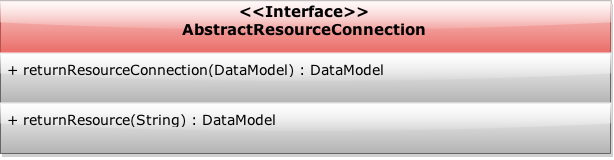
\includegraphics[scale=0.5]{Abstract_Resource_Connection_Interface.png}
	\caption{Interface AbstractResourceConnectionInterface UML Diagram}
	\label{fig:@=connection}
\end{figure}
Parameters for interface are respectively: List of Strings and String. Parameter types should be sufficient for particular data source invocation composition (e.g SQL statement). Using String type give user big flexibility if we are considering Java as programming language.
\subsection{Class \newline loadstone.api.classification.loadstone.\newline LoadstonePreprocessing}
This class is deliberately delegated to pre-process data obtained from \textit{Loadstone} database. Using dedicated interface it assures final user about possibility of preprocessing in easy to use and in the same time customized way. Class architecture is shown on \ref{fig:@=LoadstonePreprocessing}.
\begin{figure}[h]
	\centering
	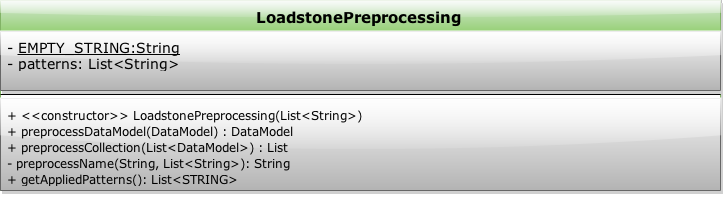
\includegraphics[scale=0.5]{LoadstonePreprocessing.png}
	\caption{LoadstonePreprocessing UML Diagram}
	\label{fig:@=LoadstonePreprocessing}
\end{figure}
Class organization is simple. For preprocessing functionality is responsible private method used in methods implementation of AbstractResourcePreprocessing interface. It simply process given input - rejects spaces (default behaviour) and patterns defined by user in constructor. Method is applied for single object DataModel or collection of such objects in corresponding interface methods.
\subsection{Class \newline loadstone.api.classification.loadstone.LoadstoneBOW}
\label{loadstone_bow}
This class is a feature for semi-supervised classification. It is basically a hashmap which values are sections of NACE categorization system and keys are strings which were the most frequent occurring in Loadstone database and assigned empirically to particular category. This class avails user traversing through map and check if category can be assigned immediately. Empirically assigned categories to BOW are presented in table: \ref{tab:BowMatching} \textbf{(it is sample of implementation)}.
\begin{table}
	\centering 
	\begin{tabular}{ | c | c |}
		\hline   
		Category  & BOW member\tabularnewline \hline
		bankomat  & K\\\hline
		kościół & U\\\hline
		kurier&J\\\hline
		pgp & J\\\hline
		szkoła & P\\\hline
		atm & K\\\hline
		cmentarz & U\\\hline
		supermarket & G\\\hline
		apteka & Q\\\hline
		bank & K\\\hline
		krzyż & U\\\hline
		most & H\\\hline
		spożywczy & I\\\hline
		restauracja & I\\\hline
		sklep & G\\\hline
		plac & H\\\hline
		hotel & I\\\hline
		euronet & K\\\hline
		bunkier & R\\\hline
		pomnik & R\\\hline
		jezioro & A\\\hline
		poczta & J\\\hline
		rynek & A\\\hline
		jedzenie & I\\\hline
		katolicki & U\\\hline
		pko & K\\\hline
		samochodowy & G\\\hline
		warsztat & G\\\hline
		szlak & A\\\hline
		biedronka & G\\\hline
		orlen & D\\\hline
		lpg & D\\\hline
		straż & O\\\hline
		myjnia & T\\\hline
	\end{tabular}
	\caption{BOW for loadstone database keywords assignments to categories}
	\label{tab:BowMatching}
\end{table} 

\subsection{Class \newline loadstone.api.classification.NaiveClassifier}
\label{naive_classifier}
This class is implementing naive classification basing on descriptions from NACE categories class (table \ref{tab:NaceMatching}) using Classifier interface. It analyses if data model name contains word which is included in particular category description. If data model name contains two or more words from distinct categories descriptions both of them are returned as possible categories to be assigned (under the condition these words have the same number of occurrence). In case of non-homogeneous phrases occurrence from distinct categories only this category is returned which was assigned to word with highest value of occurrences. This class is basing only on heuristic of NACE categories descriptions so can be used for any data source but categorization correctness may differ significantly on input data. 

\subsection{Class \newline loadstone.api.classification.loadstone.\newline LoadstoneSemiSupervisedClassifier}
\label{semi_desc}
Class which enables to classify POI using class LoadstoneBOW prepared previously. This class does not include descriptions from NACE categories descriptions (table \ref{tab:NaceMatching}). Only descriptions from LoadstoneBOW (table \ref{tab:BowMatching}) are taken into consideration. The rule of assignment to category is the same as in case of NaiveClassifier, so multiple categories can be returned as a result. This class is implementing Classifier interface so it can be fluently used later in API.

\subsection{Class \newline loadstone.api.connection.loadstone.LoadstoneDatabase}
This class takes responsibility for gathering Loadstone database. This class is implementing AbstractResourceConnection to get all possible entities from Loadstone database. 

\subsubsection{LoadstoneDatabaseUpdater Singleton Design Pattern}
To modify data inside database loadstone.api.connection.loadstone.LoadstoneDatabaseUpdater should be used. It is using Singleton pattern to assure atomicity of operation on database. It defines static method \textit{getObjectModelSingleton()} returns static object on which user can work to modify data. Such approach allows for data correctness without bothering some other object is using database.  

\subsection{Class loadstone.api.utils.LoadstoneAPIUtils}
This class is just utility for user to construct appropriate SQL query to Loadstone database. This utility only expect from user to input patterns which are supposed to be included during search for expected tuples in database. 

\subsection{Class loadstone.api.CategorizationAPI}
Class which can be enabled for final usage by user. It combines all methods of preprocessing, data source connection and classification methods. Should be used as input point for data considered to be classified and methods used for classification. Optionally user can add preprocessing method if step of this kind may be useful when POI classification is done. UML diagram on figure \ref{fig:@=CategorizationAPI}

\begin{figure}[h]
	\centering
	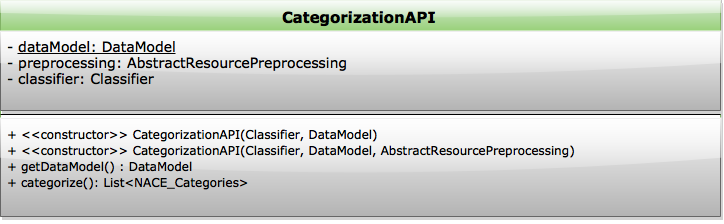
\includegraphics[scale=0.5]{CategorizationAPI.png}
	\caption{CategorizationAPI UML Diagram}
	\label{fig:@=CategorizationAPI}
\end{figure}

\section{Library Usage}
Product of created information system is API which can be used by programmer. Usage of library is simple and intuitive. Access to data source and semi-supervised classification task can be done in couple of lines in Java code. The following code snippet demonstrates how to execute categorization task using Loadstone database as data source. Chosen source data is first selected entry given by SQL query to database, contains phrase \textit{bankomat} and will be preprocessed from phrases: \textit{"ul.","adres" and "."}
\begin{lstlisting}[style=JAVA]
//define query condition
patternsToLookForInLoadstoneDatabase = new ArrayList<>();
patternsToLookForInLoadstoneDatabase.add("bankomat");
//patterns preparation for preprocessing
patternsToBeTrimmedFromConsideredDataModel = new ArrayList();
patternsToBeTrimmedFromConsideredDataModel.add("ul.");
patternsToBeTrimmedFromConsideredDataModel.add("adres");
patternsToBeTrimmedFromConsideredDataModel.add("\\.");
//Return data from database
List<DataModel> dataModels = new LoadstoneDatabase().returnResourceCollection(patternsToLookForInLoadstoneDatabase);
//takes first database entry satisfying query condition
dataModelConsidered = dataModels.get(0);
//Initial conditions for API - classification method, data source, preprocessing conditions
CategorizationAPI categorizationAPI = new CategorizationAPI(new LoadstoneSemiSupervisedClassifier(), dataModelConsidered,
new LoadstonePreprocessing(patternsToBeTrimmedFromConsideredDataModel));
//Execute categorization
List<NACE_Categories> nace_categories = categorizationAPI.categorize();
\end{lstlisting}